\documentclass[12pt,addpoints]{repaso}
\grado{6}
\nivel{Primaria}
\cicloescolar{2024-2025}
\materia{Matemáticas}
\unidad{1}
\title{Practica la Unidad}
\aprendizajes{\scriptsize%
% \item Estudio de los números.
\item Expresa oralmente la sucesión numérica hasta billones, en español y hasta donde sea posible, en su lengua materna, de manera ascendente y descendente a partir de un número natural dado. Ordena, lee y escribe números naturales de más de nueve cifras e interpreta números decimales en diferentes contextos. Identifica semejanzas y diferencias entre el sistema de numeración decimal y otros sistemas como el maya y el romano\\[-1.5em]
	% \item Suma y resta, su relación como operaciones inversas.
	\item A partir de situaciones problemáticas vinculadas a diferentes contextos, suma y resta números decimales y fracciones con diferentes denominadores.\\[-1.5em]
	% \item Multiplicación y división, su relación como operaciones inversas.
	\item Resuelve situaciones problemáticas vinculadas a diferentes contextos que implican dividir números decimales entre naturales. También, dividir números fraccionarios entre números naturales.\\[-1.5em]
	% \item Relaciones de proporcionalidad.
	\item A partir de situaciones problemáticas de proporcionalidad vinculadas a diferentes contextos, determina valores faltantes en las que en ocasiones se conoce el valor unitario y en otras no.\\[-1.5em]
	% \item Ubicación espacial.
	\item Lee, interpreta y elabora planos para comunicar la ubicación de seres vivos y objetos.\\[-1.5em]
	% \item Figuras y cuerpos geométricos y sus características.
	\item Explora y reconoce las características del cilindro y cono; anticipa y comprueba desarrollos planos que permiten construirlos.\\[-1.5em]
	% \item Perímetro, área y noción de volumen.
	\item Resuelve situaciones problemáticas que implican calcular el perímetro y área de figuras compuestas por triángulos y cuadriláteros. Resuelve problemas que implican construir, estimar y comparar el volumen de cuerpos y prismas rectos rectangulares mediante el conteo de cubos, y reconoce que existen diferentes cuerpos con el mismo volumen.\\[-1.5em]
	% \item Organización e interpretación de datos.
	\item Interpreta información cuantitativa y cualitativa contenida en tablas, gráficas de barras y circulares para responder preguntas vinculadas a diferentes contextos; construye gráficas de barras. Genera y organiza datos, determina la moda, la media aritmética y el rango para responder preguntas vinculadas a diferentes contextos.\\[-1.5em]
	% \item Nociones de probabilidad.
	\item Clasifica eventos de diversos contextos utilizando términos como seguro, imposible, probable, muy probable o poco probable que sucedan.
}
\author{Melchor Pinto, JC}
\begin{document}
\INFO\afterpage{\blankpage}
\begin{multicols}{2}
	\tableofcontents
\end{multicols}
\begin{questions}\large
	\addcontentsline{toc}{section}{Unidad 1}
	\section*{Unidad 1}

	\addcontentsline{toc}{subsection}{Sumas y restas}
	\subsection*{Sumas y restas}

	% \addcontentsline{toc}{subsubsection}{Sumas 1}
	% \subsubsection*{Sumas 1}
	% \addcontentsline{toc}{subsubsection}{Sumas 2}
	% \subsubsection*{Sumas 2}
	% \addcontentsline{toc}{subsubsection}{Restas 1}
	% \subsubsection*{Restas 1}
	% \addcontentsline{toc}{subsubsection}{Restas 2}
	% \subsubsection*{Restas 2}
	\questionboxed[2]{Realiza las siguientes sumas y restas:

		\begin{multicols}{4}
			\begin{parts}
				\part
				\ifprintanswers{\opadd[hfactor=decimal,resultstyle=\color{red},carryadd=true]{17}{18}}
				\else{\opadd[hfactor=decimal,resultstyle=\color{white},carryadd=false]{17}{18}\\[0.5cm]}\fi

				\part
				\ifprintanswers{\opadd[hfactor=decimal,resultstyle=\color{red},carryadd=true]{1155}{893}}
				\else{\opadd[hfactor=decimal,resultstyle=\color{white},carryadd=false]{1155}{893}\\[0.5cm]}\fi

				\part
				\ifprintanswers{\opadd[hfactor=decimal,resultstyle=\color{red},carryadd=true]{26}{19}}
				\else{\opadd[hfactor=decimal,resultstyle=\color{white},carryadd=false]{26}{19}}\fi

				\part
				\ifprintanswers{\opadd[hfactor=decimal,resultstyle=\color{red},carryadd=true]{2271}{1028}}
				\else{\opadd[hfactor=decimal,resultstyle=\color{white},carryadd=false]{2271}{1028}\\[0.5cm]}\fi

				\part
				\ifprintanswers{\opadd[hfactor=decimal,resultstyle=\color{red},carryadd=true]{182}{149}}
				\else{\opadd[hfactor=decimal,resultstyle=\color{white},carryadd=false]{182}{149}\\[0.5cm]}\fi

				\part
				\ifprintanswers{\opadd[hfactor=decimal,resultstyle=\color{red},carryadd=true]{7449}{4358}}
				\else{\opadd[hfactor=decimal,resultstyle=\color{white},carryadd=false]{7449}{4358}}\fi

				\part \ifprintanswers{   \opsub[hfactor=decimal,resultstyle=\color{red},carryadd=true,carrysub=true]{706}{589} }
				\else{            \opsub[hfactor=decimal,resultstyle=\color{white},carryadd=false,carrysub=false]{706}{589}\\[0.5cm] }
				\fi

				\part \ifprintanswers{   \opsub[hfactor=decimal,resultstyle=\color{red},carryadd=true,carrysub=true]{3004}{1242} }
				\else{            \opsub[hfactor=decimal,resultstyle=\color{white},carryadd=false,carrysub=false]{3004}{1242}\\[0.5cm] }
				\fi

				\part \ifprintanswers{   \opsub[hfactor=decimal,resultstyle=\color{red},carryadd=true,carrysub=true]{1600}{669} }
				\else{            \opsub[hfactor=decimal,resultstyle=\color{white},carryadd=false,carrysub=false]{1600}{669} }
				\fi

				\part \ifprintanswers{   \opsub[hfactor=decimal,resultstyle=\color{red},carryadd=true,carrysub=true]{4005}{2831} }
				\else{            \opsub[hfactor=decimal,resultstyle=\color{white},carryadd=false,carrysub=false]{4005}{2831}\\[0.5cm] }
				\fi

				\part \ifprintanswers{   \opsub[hfactor=decimal,resultstyle=\color{red},carryadd=true,carrysub=true]{1200}{966} }
				\else{            \opsub[hfactor=decimal,resultstyle=\color{white},carryadd=false,carrysub=false]{1200}{966} \\[0.5cm]}
				\fi

				% \part \ifprintanswers{   \opsub[hfactor=decimal,resultstyle=\color{red},carryadd=true,carrysub=true]{42784}{34180} }
				% \else{            \opsub[hfactor=decimal,resultstyle=\color{white},carryadd=false,carrysub=false]{42784}{34180} \\[0.5cm]}
				% \fi

				\part \ifprintanswers{   \opsub[hfactor=decimal,resultstyle=\color{red},carryadd=true,carrysub=true]{800}{744} }
				\else{            \opsub[hfactor=decimal,resultstyle=\color{white},carryadd=false,carrysub=false]{800}{744} }
				\fi

				% \part \ifprintanswers{   \opsub[hfactor=decimal,resultstyle=\color{red},carryadd=true,carrysub=true]{37881}{24049} }
				% \else{            \opsub[hfactor=decimal,resultstyle=\color{white},carryadd=false,carrysub=false]{37881}{24049}\\[0.5cm] }
				% \fi
			\end{parts}
		\end{multicols}
	}

	% \addcontentsline{toc}{subsubsection}{Resolución de problemas}
	% \subsubsection*{Resolución de problemas}

	\questionboxed[2]{Resuelve los siguientes problemas sobre sumas y restas:

		\begin{multicols}{2}
			\begin{parts}
				% \part El total de mis compras es de 315 pesos, ¿cuánto dinero recibiré de cambio si pago con un billete de 500 pesos?

				% \begin{solutionbox}{1cm}
				% 	\opsub[style=text]{500}{315}
				% \end{solutionbox}

				% \part Luis tiene ahorrado 257 pesos, si su abuelo le regala 360 pesos más, ¿cuánto dinero tiene en total Luis?

				% \begin{solutionbox}{1cm}
				% 	\opadd[style=text]{257}{360}
				% \end{solutionbox}

				\part Jorge está armando un rompecabezas de 500 piezas, si ha puesto 233 piezas, ¿cuántas piezas le faltan por poner a Jorge?

				\begin{solutionbox}{1cm}
					\opsub[style=text]{500}{233}
				\end{solutionbox}

				\part Carlos mide 183 centímetros y es 8 centímetros más alto que Julio, ¿cuántos centímetros mide Julio?

				\begin{solutionbox}{1cm}
					\opsub[style=text]{183}{8}
				\end{solutionbox}
			\end{parts}
		\end{multicols}
	}



	\addcontentsline{toc}{subsection}{Multiplicaciones y divisiones}
	\subsection*{Multiplicaciones y divisiones}



	% \addcontentsline{toc}{subsubsection}{Multiplicaciones 1}
	% \subsubsection*{Multiplicaciones 1}
	% \addcontentsline{toc}{subsubsection}{Multiplicaciones 2}
	% \subsubsection*{Multiplicaciones 2}
	\questionboxed[2]{Realiza las siguientes multiplicaciones:

		\begin{multicols}{3}
			\begin{parts}
				\part \ifprintanswers{\normalsize\opmul[hfactor=decimal,resultstyle=\color{red},displayintermediary=None]{314}{2} }
				\else{\normalsize\opmul[hfactor=decimal,resultstyle=\color{white},displayintermediary=None]{314}{2}}\\[2em]\fi

				\part \ifprintanswers{\normalsize\opmul[hfactor=decimal,resultstyle=\color{red},displayintermediary=all]{283}{44} }
				\else{\normalsize\opmul[hfactor=decimal,resultstyle=\color{white},displayintermediary=None]{283}{44}}\fi

				\part \ifprintanswers{\normalsize\opmul[hfactor=decimal,resultstyle=\color{red},displayintermediary=None]{2781}{5} }
				\else{\normalsize\opmul[hfactor=decimal,resultstyle=\color{white},displayintermediary=None]{2781}{5}}\\[2em]\fi

				\part \ifprintanswers{\normalsize\opmul[hfactor=decimal,resultstyle=\color{red},displayintermediary=all]{3914}{106} }
				\else{\normalsize\opmul[hfactor=decimal,resultstyle=\color{white},displayintermediary=None]{3914}{106}}\fi

				\part \ifprintanswers{\normalsize\opmul[hfactor=decimal,resultstyle=\color{red},displayintermediary=all]{255}{24} }
				\else{\normalsize\opmul[hfactor=decimal,resultstyle=\color{white},displayintermediary=None]{255}{24}}\\[2em]\fi

				\part \ifprintanswers{\normalsize\opmul[hfactor=decimal,resultstyle=\color{red},displayintermediary=all]{3533}{29} }
				\else{\normalsize\opmul[hfactor=decimal,resultstyle=\color{white},displayintermediary=None]{3533}{29}}\fi
			\end{parts}
		\end{multicols}
	}

	% \addcontentsline{toc}{subsubsection}{Resolución de problemas}
	% \subsubsection*{Resolución de problemas}
	\questionboxed[2]{Resuelve los siguientes problemas sobre multiplicaciones:

		\begin{multicols}{2}
			\begin{parts}
				\part Una escuela tiene 6 salones, si cada salón tiene 25 alumnos. ¿Cuántos alumnos tiene en total la escuela?

				\begin{solutionbox}{1cm}
					\opmul[style=text]{6}{25}
				\end{solutionbox}

				\part Una cubeta de pintura cuesta 2345 pesos, ¿cuánto se pagará por 3 cubetas de pintura?

				\begin{solutionbox}{1cm}
					\opmul[style=text]{3}{2345}
				\end{solutionbox}

				\part Una secretaria puede escribir 36 palabras por minuto si continua con este ritmo, ¿cuántas palabras puede escribir en 12 minutos?

				\begin{solutionbox}{1cm}
					\opmul[style=text]{36}{12}
				\end{solutionbox}

				\part Cristina compró 5 cajas de leche de soya, si cada caja tiene 12 envases de leche, ¿cuántos envases de leche compró Cristina?

				\begin{solutionbox}{1cm}
					\opmul[style=text]{5}{12}
				\end{solutionbox}

				\part Mariana fue a la frutería y compró 3 kilogramos de uvas, si el kilogramo cuesta 84 pesos. ¿Cuánto pagó en total Mariana?

				\begin{solutionbox}{1cm}
					\opmul[style=text]{3}{84}
				\end{solutionbox}

				\part Laura compró 28 paquetes de galletas, si cada paquete tiene 18 galletas. ¿Cuántas galletas tiene en total Laura?

				\begin{solutionbox}{1cm}
					\opmul[style=text]{28}{18}
				\end{solutionbox}

			\end{parts}
		\end{multicols}
	}

	% \addcontentsline{toc}{subsubsection}{Divisiones 1}
	% \subsubsection*{Divisiones 1}
	% \addcontentsline{toc}{subsubsection}{Divisiones 2}
	% \subsubsection*{Divisiones 2}

	\questionboxed[2]{Calcula el {\color{red}cociente} y {\color{blue} residuo} de las siguientes divisiones de números enteros:

		\begin{multicols}{4}
			\begin{parts}
				\part \ifprintanswers{\opidiv[resultstyle=\color{red},remainderstyle.1=\color{blue!100!white}]{23}{6}} \\[2em]
				\else{           $6 \overline{) \ 23\ }$} \\[4em]
				\fi

				\part \ifprintanswers{\opidiv[resultstyle=\color{red},remainderstyle.2=\color{blue!100!white}]{200}{3}} \\[2em]
				\else{           $3 \overline{) \ 200\ }$} \\[4em]
				\fi

				\part \ifprintanswers{\opidiv[resultstyle=\color{red},remainderstyle.2=\color{blue!100!white}]{99}{8}} \\[2em]
				\else{           $8 \overline{) \ 99\ }$} \\[4em]
				\fi

				\part \ifprintanswers{\opidiv[resultstyle=\color{red},remainderstyle.2=\color{blue!100!white}]{283}{6}} \\[2em]
				\else{           $6 \overline{) \ 283\ }$} \\[4em]
				\fi

				\part \ifprintanswers{\opidiv[resultstyle=\color{red},remainderstyle.3=\color{blue!100!white}]{4032}{8}} \\[2em]
				\else{           $8 \overline{) \ 4032\ }$} \\[4em]
				\fi

				\part \ifprintanswers{\opidiv[resultstyle=\color{red},remainderstyle.2=\color{blue!100!white}]{644}{8}} \\[2em]
				\else{           $8 \overline{) \ 644\ }$} \\[4em]
				\fi

				\part \ifprintanswers{\opidiv[resultstyle=\color{red},remainderstyle.2=\color{blue!100!white}]{656}{7}} \\[2em]
				\else{           $7 \overline{) \ 656\ }$} \\[4em]
				\fi

				\part \ifprintanswers{\opidiv[resultstyle=\color{red},remainderstyle.3=\color{blue!100!white}]{2303}{7}} \\[2em]
				\else{           $7 \overline{) \ 2303\ }$} \\[4em]
				\fi
			\end{parts}
		\end{multicols}
	}




	\addcontentsline{toc}{subsection}{Números decimales}
	\subsection*{Números decimales}
	% \addcontentsline{toc}{subsubsection}{Posición decimal y notación desarrollada}
	% \subsubsection*{Posición decimal y notación desarrollada}


	\questionboxed[2]{Señala la opción que responda correctamente a cada una de las siguientes preguntas:

		\begin{multicols}{2}
			\begin{parts}
				\part En el número 1.829, ¿qué número ocupa la posición de las centésimas?

				\begin{oneparcheckboxes}
					\choice 1 \CorrectChoice 2 \choice 6 \choice 8 \choice 9
				\end{oneparcheckboxes}

				\part En el número 2.087, ¿qué número ocupa la posición de las décimas?

				\begin{oneparcheckboxes}
					\CorrectChoice 0 \choice 2 \choice 7 \choice 8 \choice 9
				\end{oneparcheckboxes}

				\part En el número 5.928, ¿qué número ocupa la posición de las décimas?

				\begin{oneparcheckboxes}
					\choice 5 \choice 2 \choice 6 \choice 8 \CorrectChoice 9
				\end{oneparcheckboxes}

				\part En el número 3.284, ¿qué número ocupa la posición de las milésimas?

				\begin{oneparcheckboxes}
					\choice 2 \choice 3 \CorrectChoice 4  \choice 8 \choice 9
				\end{oneparcheckboxes}

				\part En el número 1.285, ¿qué número ocupa la posición de las décimas?

				\begin{oneparcheckboxes}
					\choice 1 \CorrectChoice 2 \choice 5 \choice 8 \choice 9
				\end{oneparcheckboxes}

				\part En el número 1.823, ¿qué número ocupa la posición de las milésimas?

				\begin{oneparcheckboxes}
					\choice 1 \choice 2 \CorrectChoice 3 \choice 6 \choice 8
				\end{oneparcheckboxes}
			\end{parts}
		\end{multicols}
	}

	% \addcontentsline{toc}{subsubsection}{Decimales en la recta numérica}
	% \subsubsection*{Decimales en la recta numérica}

	\questionboxed[2]{Escribe en el recuadro el número decimal que representa el punto en la recta numérica de cada imagen:

		\begin{multicols}{2}
			\begin{parts}
				\part 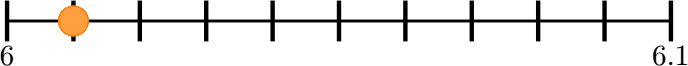
\includegraphics[width=180px]{../images/recta_num_6.01.png}  \hfill \fillin[\fbox{6.01}][0in] \\
				% \part 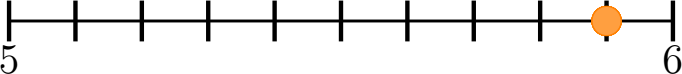
\includegraphics[width=180px]{../images/recta_num_5.9.png}   \hfill \fillin[\fbox{5.9 }][0in] \\
				\part 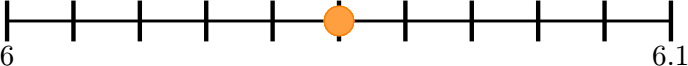
\includegraphics[width=180px]{../images/recta_num_6.05.png}  \hfill \fillin[\fbox{6.05}][0in] \\
				\part 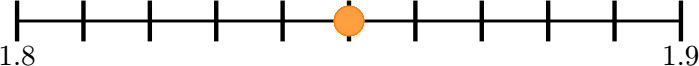
\includegraphics[width=180px]{../images/recta_num_1.85.png}  \hfill \fillin[\fbox{1.85}][0in] \\
				% \part 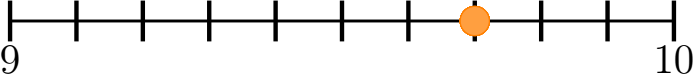
\includegraphics[width=180px]{../images/recta_num_9.7.png}   \hfill \fillin[\fbox{9.7 }][0in] \\
				\part 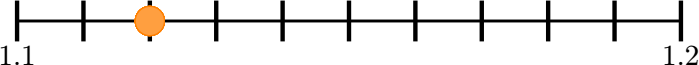
\includegraphics[width=180px]{../images/recta_num_1.12.png}  \hfill \fillin[\fbox{1.12}][0in] \\
				\part 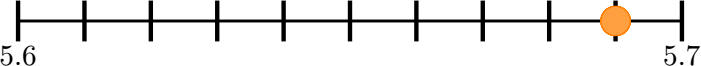
\includegraphics[width=180px]{../images/recta_num_5.69.png}  \hfill \fillin[\fbox{5.69}][0in] \\
				% \part 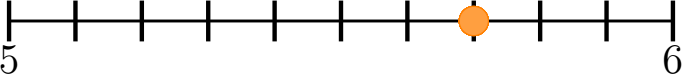
\includegraphics[width=180px]{../images/recta_num_5.7.png}   \hfill \fillin[\fbox{5.7 }][0in] \\
				\part 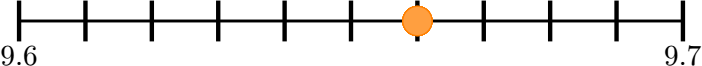
\includegraphics[width=180px]{../images/recta_num_9.66.png}  \hfill \fillin[\fbox{9.66}][0in] \\
				% \part 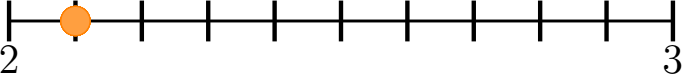
\includegraphics[width=180px]{../images/recta_num_2.1.png}   \hfill \fillin[\fbox{2.1 }][0in] \\
			\end{parts}
		\end{multicols}
	}

	% \addcontentsline{toc}{subsubsection}{Nombre de decimales}
	% \subsubsection*{Nombre de decimales}
	\questionboxed[2]{Escribe los siguientes números

		\begin{multicols}{2}
			\begin{parts}\normalsize
				% \part Catorce enteros diecinueve centésimos 	\hfill \fillin[14.19][1.2cm]
				\part Cuatro enteros once diez milésimos 		\hfill \fillin[4.0011][1.2cm]
				% \part Seis enteros setenta y dos centésimos 	\hfill \fillin[6.72][1.2cm]
				% \part Siete enteros novecientos tres milésimos 	\hfill \fillin[7.903][1.2cm]
				% \part Seis enteros doscientos trece milésimos 	\hfill \fillin[6.213][1.2cm]
				% \part Cincuenta enteros cinco décimos 			\hfill \fillin[50.5][1.2cm]
				\part Nueve enteros cuatro centésimos 			\hfill \fillin[9.04][1.2cm]
				% \part Cuatro enteros setecientos doce milésimos \hfill \fillin[4.712][1.2cm]
				\part Seis mil catorce diez milésimos 			\hfill \fillin[0.6014][1.2cm]
				% \part Nueve enteros once centésimos 			\hfill \fillin[9.11][1.2cm]
				% \part Cuarenta enteros cuatro centésimos 		\hfill \fillin[40.04][1.2cm]
				% \part Dieciocho enteros siete décimos 			\hfill \fillin[18.7][1.2cm]
				% \part Veinte enteros tres décimos 				\hfill \fillin[20.3][1.2cm]
				\part Cuatro enteros ciento dos diez milésimos 	\hfill \fillin[4.0102][1.2cm]
				% \part Ocho enteros trece diez milésimos 		\hfill \fillin[8.0013][1.2cm]
			\end{parts}
		\end{multicols}
	}

	

	%%% \addcontentsline{toc}{subsubsection}{Comparación de decimales}
	%%% \subsubsection*{Comparación de decimales}
	%%% \addcontentsline{toc}{subsubsection}{Redondeo de decimales}
	%%% \subsubsection*{Redondeo de decimales}

	\questionboxed[2]{\textbf{Redondea} los siguientes números decimales como se pide:

		\begin{multicols}{2}
			\begin{parts}\normalsize
				\part $8.0375 $ a la milésima más cercana       \hfill \fillin[$8.038 $][1.2cm]
				% \part $3.09628$ a la diez milésima más cercana  \hfill \fillin[$3.0963$][1.2cm]
				% \part $3.28   $ a la décima más cercana         \hfill \fillin[$3.3   $][1.2cm]
				% \part $5.308  $ a la centésima más cercana      \hfill \fillin[$5.31  $][1.2cm]
				% \part $8.57   $ a la décima más cercana         \hfill \fillin[$8.6   $][1.2cm]
				% \part $7.229  $ a la décima más cercana         \hfill \fillin[$7.2   $][1.2cm]
				% \part $9.85713$ a la milésima más cercana       \hfill \fillin[$9.857 $][1.2cm]
				% \part $6.12   $ a la décima más cercana         \hfill \fillin[$6.1   $][1.2cm]
				% \part $3.4952 $ a la milésima más cercana       \hfill \fillin[$3.495 $][1.2cm]
				% \part $2.52   $ a la décima más cercana         \hfill \fillin[$2.5   $][1.2cm]
				\part $6.28629$ a la diez milésima más cercana  \hfill \fillin[$6.2863$][1.2cm]
				\part $1.9286 $ a la milésima más cercana       \hfill \fillin[$1.929 $][1.2cm]
				% \part $4.27   $ a la décima más cercana         \hfill \fillin[$4.3   $][1.2cm]
				% \part $3.4025 $ a la décima más cercana         \hfill \fillin[$3.4   $][1.2cm]
				\part $5.03751$ a la milésima más cercana       \hfill \fillin[$5.038 $][1.2cm]
			\end{parts}
		\end{multicols}
	}

	\addcontentsline{toc}{subsection}{Operaciones con decimales}
	\subsection*{Operaciones con decimales}
	% \addcontentsline{toc}{subsubsection}{Suma de decimales}
	% \subsubsection*{Suma de decimales}

	\questionboxed[2]{Realiza las siguientes sumas con números decimales:

		\begin{multicols}{3}
			\begin{parts}
				\part \ifprintanswers{   \opadd[hfactor=decimal,resultstyle=\color{red},carryadd=true,carrysub=false]{24.34}{13.84} }
				\else{            \opadd[hfactor=decimal,resultstyle=\color{white},carryadd=false,carrysub=false]{24.34}{13.84}\\[0.5cm]}
				\fi

				\part \ifprintanswers{   \opadd[hfactor=decimal,resultstyle=\color{red},carryadd=true,carrysub=false]{684.99}{583.82} }
				\else{           \opadd[hfactor=decimal,resultstyle=\color{white},carryadd=false,carrysub=false]{684.99}{583.82} }
				\fi

				\part \ifprintanswers{   \opadd[hfactor=decimal,resultstyle=\color{red},carryadd=true,carrysub=false]{51.238}{34.993} }
				\else{            \opadd[hfactor=decimal,resultstyle=\color{white},carryadd=false,carrysub=false]{51.238}{34.993}\\[0.5cm] }
				\fi

				\part \ifprintanswers{   \opadd[hfactor=decimal,resultstyle=\color{red},carryadd=true,carrysub=false]{90.371}{45.392} }
				\else{            \opadd[hfactor=decimal,resultstyle=\color{white},carryadd=false,carrysub=false]{90.371}{45.392} }
				\fi

				\part \ifprintanswers{   \opadd[hfactor=decimal,resultstyle=\color{red},carryadd=true,carrysub=false]{18.03}{7.45} }
				\else{            \opadd[hfactor=decimal,resultstyle=\color{white},carryadd=false,carrysub=false]{18.03}{7.45}\\[0.5cm] }
				\fi

				\part \ifprintanswers{   \opadd[hfactor=decimal,resultstyle=\color{red},carryadd=true,carrysub=false]{9.931}{5.198} }
				\else{           \opadd[hfactor=decimal,resultstyle=\color{white},carryadd=false,carrysub=false]{9.931}{5.198} }
				\fi
			\end{parts}
		\end{multicols}
	}

	% \addcontentsline{toc}{subsubsection}{Resta de decimales}
	% \subsubsection*{Resta de decimales}

	\questionboxed[2]{Realiza las siguientes restas con números decimales:

		\begin{multicols}{3}
			\begin{parts}
				\part \ifprintanswers{   \opsub[hfactor=decimal,resultstyle=\color{red},carryadd=true,carrysub=true]{9.754}{3.862} }
				\else{            \opsub[hfactor=decimal,resultstyle=\color{white},carryadd=false,carrysub=false]{9.754}{3.862}\\[0.5cm]}
				\fi

				\part \ifprintanswers{   \opsub[hfactor=decimal,resultstyle=\color{red},carryadd=true,carrysub=true]{1.668}{1.464} }
				\else{            \opsub[hfactor=decimal,resultstyle=\color{white},carryadd=false,carrysub=false]{1.668}{1.464} }
				\fi

				\part \ifprintanswers{   \opsub[hfactor=decimal,resultstyle=\color{red},carryadd=true,carrysub=true]{4.298}{3.465} }
				\else{            \opsub[hfactor=decimal,resultstyle=\color{white},carryadd=false,carrysub=false]{4.298}{3.465}\\[0.5cm] }
				\fi

				\part \ifprintanswers{   \opsub[hfactor=decimal,resultstyle=\color{red},carryadd=true,carrysub=true]{90.371}{45.392} }
				\else{            \opsub[hfactor=decimal,resultstyle=\color{white},carryadd=false,carrysub=false]{90.371}{45.392} }
				\fi

				\part \ifprintanswers{   \opsub[hfactor=decimal,resultstyle=\color{red},carryadd=true,carrysub=true]{16.03}{6.45} }
				\else{            \opsub[hfactor=decimal,resultstyle=\color{white},carryadd=false,carrysub=false]{16.03}{6.45}\\[0.5cm] }
				\fi

				\part \ifprintanswers{   \opsub[hfactor=decimal,resultstyle=\color{red},carryadd=true,carrysub=true]{6.231}{2.188} }
				\else{            \opsub[hfactor=decimal,resultstyle=\color{white},carryadd=false,carrysub=false]{6.231}{2.188} }
				\fi
			\end{parts}
		\end{multicols}
	}
	% \addcontentsline{toc}{subsubsection}{Multiplicación de decimales}
	% \subsubsection*{Multiplicación de decimales}

	\questionboxed[2]{Realiza las siguientes multiplicaciones con números decimales:

		\begin{multicols}{3}
			\begin{parts}
				\part \ifprintanswers{\normalsize\opmul[hfactor=decimal,resultstyle=\color{red},displayintermediary=None]{3.24}{2.52} }
				\else{\opmul[hfactor=decimal,resultstyle=\color{white},displayintermediary=None]{3.24}{2.52}}\\[2em]\fi

				\part \ifprintanswers{\normalsize\opmul[hfactor=decimal,resultstyle=\color{red},displayintermediary=all]{7.75}{3.8} }
				\else{\opmul[hfactor=decimal,resultstyle=\color{white},displayintermediary=None]{7.75}{3.8}}\\[2em]\fi

				\part \ifprintanswers{\normalsize\opmul[hfactor=decimal,resultstyle=\color{red},displayintermediary=None]{1.9}{1.2} }
				\else{\opmul[hfactor=decimal,resultstyle=\color{white},displayintermediary=None]{1.9}{1.2}}\\[2em]\fi

				\part \ifprintanswers{\normalsize\opmul[hfactor=decimal,resultstyle=\color{red},displayintermediary=all]{2.5}{2.3} }
				\else{\opmul[hfactor=decimal,resultstyle=\color{white},displayintermediary=None]{2.5}{2.3}}\\[2em]\fi

				\part \ifprintanswers{\normalsize\opmul[hfactor=decimal,resultstyle=\color{red},displayintermediary=all]{23.4}{8.5} }
				\else{\opmul[hfactor=decimal,resultstyle=\color{white},displayintermediary=None]{23.4}{8.5}}\\[2em]\fi

				\part \ifprintanswers{\normalsize\opmul[hfactor=decimal,resultstyle=\color{red},displayintermediary=all]{5.3}{1.6} }
				\else{\opmul[hfactor=decimal,resultstyle=\color{white},displayintermediary=None]{5.3}{1.6}}\\[2em]\fi
			\end{parts}
		\end{multicols}
	}


	%%% \addcontentsline{toc}{subsubsection}{División de decimales}
	%%% \subsubsection*{División de decimales}

	\questionboxed[2]{Calcula el resultado de las siguientes divisiones de números decimales:

		\opset{strikedecimalsepsymbol={\rlap{,}\rule[-1pt]{3pt}{0.4pt}}}
		\begin{multicols}{4}
			\begin{parts}
				\part \ifprintanswers{\opdiv[shiftdecimalsep=divisor,strikedecimalsepsymbol=\hspace{-2.5pt}\tiny\color{red!50!black}$\times$]{4.025}{2.3}} \\[2em]
				\else{           $2.3 \overline{) \ 4.025\ }$} \\[4em]
				\fi

				\part \ifprintanswers{\opdiv[shiftdecimalsep=divisor,strikedecimalsepsymbol=\hspace{-2.5pt}\tiny\color{red!50!black}$\times$]{17.6}{3.2}} \\[2em]
				\else{           $3.2 \overline{) \ 17.6\ }$} \\[4em]
				\fi

				\part \ifprintanswers{\opdiv[shiftdecimalsep=divisor,strikedecimalsepsymbol=\hspace{-2.5pt}\tiny\color{red!50!black}$\times$]{39}{8.125}} \\[2em]
				\else{           $8.125 \overline{) \ 39\ }$} \\[4em]
				\fi

				\part \ifprintanswers{\opdiv[shiftdecimalsep=divisor,strikedecimalsepsymbol=\hspace{-2.5pt}\tiny\color{red!50!black}$\times$]{56.1}{6.6}} \\[2em]
				\else{           $6.6 \overline{) \ 56.1\ }$} \\[4em]
				\fi
			\end{parts}
		\end{multicols}
	}

	%%% \addcontentsline{toc}{subsubsection}{Resolución de problemas}
	%%% \subsubsection*{Resolución de problemas}

	\addcontentsline{toc}{subsection}{Números decimales a fracciones}
	\subsection*{Números decimales a fracciones}
	%%% \addcontentsline{toc}{subsubsection}{Ubicación en la recta numérica}
	%%% \subsubsection*{Ubicación en la recta numérica}


	% \addcontentsline{toc}{subsubsection}{Porcentajes a decimal}
	% \subsubsection*{Porcentajes a decimal}

	\questionboxed[2]{Escribe los siguientes porcentajes como números decimales:

		\begin{multicols}{4}
			\begin{parts}
				\part $14\%=$ \fillin[\fbox{0.14}][0cm]
				\part $73\%=$ \fillin[\fbox{0.73}][0cm]
				\part $15\%=$ \fillin[\fbox{0.15}][0cm]
				\part $85\%=$ \fillin[\fbox{0.85}][0cm]
				\part $91\%=$ \fillin[\fbox{0.91}][0cm]
				\part $19\%=$ \fillin[\fbox{0.19}][0cm]
				\part $ 9\%=$ \fillin[\fbox{0.09}][0cm]
				\part $42\%=$ \fillin[\fbox{0.42}][0cm]
				\part $25\%=$ \fillin[\fbox{0.25}][0cm]
				\part $ 3\%=$ \fillin[\fbox{0.03}][0cm]
				\part $ 8\%=$ \fillin[\fbox{0.08}][0cm]
				\part $ 2\%=$ \fillin[\fbox{0.02}][0cm]
			\end{parts}
		\end{multicols}
	}

	%%% \addcontentsline{toc}{subsubsection}{Operaciones con múltiplos de 10}
	%%% \subsubsection*{Operaciones con múltiplos de 10}


	% \addcontentsline{toc}{subsubsection}{Conversión de fracciones a decimales}
	% \subsubsection*{Conversión de fracciones a decimales}

	\questionboxed[2]{Convierte las siguientes fracciones a decimal:

		\begin{multicols}{5}
			\begin{parts}
				\part $\dfrac{2}{9} =$   \fillin[\fbox{$0.\overline{2}$}][0cm]\\
				\part $\dfrac{1}{4} =$   \fillin[\fbox{$0.25$}][0cm]\\
				\part $\dfrac{2}{3} =$   \fillin[\fbox{$0.\overline{6}$}][0cm]\\
				\part $\dfrac{7}{8} =$   \fillin[\fbox{$0.875$}][0cm]\\
				\part $\dfrac{1}{9} =$   \fillin[\fbox{$0.\overline{1}$}][0cm]\\
				\part $\dfrac{6}{8} =$   \fillin[\fbox{$0.75$}][0cm]\\
				\part $\dfrac{7}{20}=$   \fillin[\fbox{$0.35$}][0cm]\\
				\part $\dfrac{5}{8} =$   \fillin[\fbox{$0.625$}][0cm]\\
				\part $\dfrac{2}{10}=$   \fillin[\fbox{$0.2$}][0cm]\\
				\part $\dfrac{5}{6} =$   \fillin[\fbox{$0.8\overline{3}$}][0cm]\\
			\end{parts}
		\end{multicols}
	}

	% \addcontentsline{toc}{subsubsection}{Conversión de decimales a fracciones}
	% \subsubsection*{Conversión de decimales a fracciones}

	\questionboxed[2]{Convierte los siguientes números decimales a una fracción simplificada a su mínima expresión:

		\begin{multicols}{4}
			\begin{parts}
				\part $0.248=$ \fillin[\fbox{$\dfrac{31}{125}$}][0cm]
				\part $0.46=$  \fillin[\fbox{$\dfrac{23}{50}$}][0cm]
				\part $0.24=$  \fillin[\fbox{$\dfrac{6}{25}$}][0cm]
				\part $0.9=$   \fillin[\fbox{$\dfrac{9}{10}$}][0cm]
				\part $0.115=$ \fillin[\fbox{$\dfrac{23}{200}$}][0cm]
				\part $0.66=$  \fillin[\fbox{$\dfrac{33}{50}$}][0cm]
				\part $0.56=$  \fillin[\fbox{$\dfrac{14}{25}$}][0cm]
				\part $0.58=$  \fillin[\fbox{$\dfrac{29}{50}$}][0cm]
			\end{parts}
		\end{multicols}
	}
\end{questions}
\end{document}